%! Author = joels
%! Date = 05/01/2021

\section{GUI Programmierung}
\subsection{View und ViewGroup}
\textcolor{blue}{View} ist die Basisklasse aller GUI Elemente. Es belegt einen rechteckigen Bereich und kümmert sich um die Darstellung und Event Verarbeitung.\\
Die Ableitung \textcolor{blue}{ViewGroup} enthält View-Objekte (Parent-Child Beziehung). ViewGroup-Klassen ordnen ihre Kinder nach einem Muster an, sind strukturierend und unsichterbar. Werden auch \textcolor{blue}{Layouts} oder \textcolor{blue}{Container} genannt.
\subsection{Layouts Allgemein}
Im onCreate der Activity wird das layout geladen:
\begin{lstlisting}
@Override
protected void onCreate(Bundle savedInstanceState) {
    super.onCreate(savedInstanceState);
    setContentView(R.layout.activity_main);
}
\end{lstlisting}
\textbf{\textcolor{blue}{Layouts Übersicht:}}\\
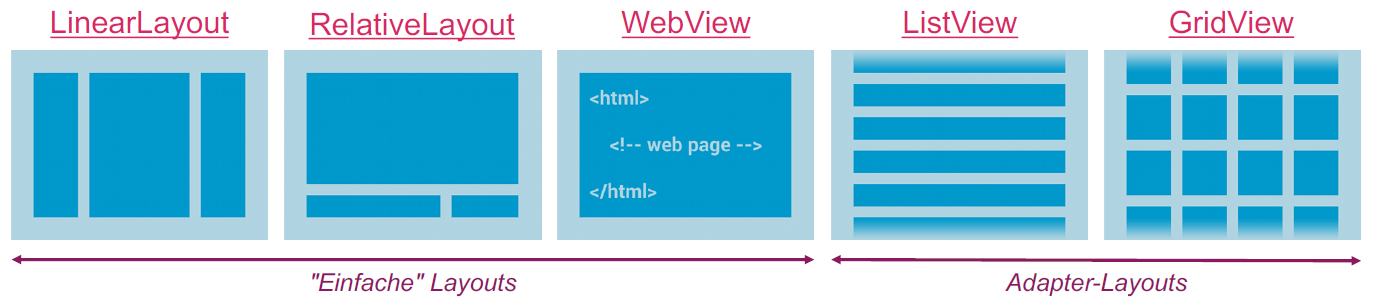
\includegraphics{layouts.png}
Es gibt noch weitere Layouts und eigene können auch definiert werden. Layouts können beliebig verschachtelt werden, jedoch mit negativem Einfluss auf die Performance. $\rightarrow$ Am besten Flache, breite Hierarchie
\subsubsection{Layout-Parameter}
Verschachtelte Child View teilt Parent mit, wie sie angeordnet werden wollen. Child setzt auf sich selber diese Parameter.
\begin{lstlisting}
<LinearLayout
    android:layout_width="match_parent"
    android:layout_height="match_parent"
    android:orientation="vertical"
    android:gravity="center">
</LinearLayout>
\end{lstlisting}
Mögliche Werte: \textcolor{blue}{match\_parent} (so gross wie möglich), \textcolor{blue}{wrap\_content} (so klein wie Content) und Zahl (unüblich, meist in dp).
\subsubsection{padding und Margin}
Padding wird auf sich selbst gesetzt. Margin wird dem Parent übergeben, da ein Child nicht einfach den Platz dem Parent wegnehmen kann.
\begin{lstlisting}
android:padding="20dp"
android:layout_margin="20dp"
\end{lstlisting}
\subsection{Linear Layout}
Vertikal oder horizontal angeordnet. Mit \textcolor{blue}{layout\_weight} kann die Grösse beeinflusst werden. $\rightarrow$ Verwendung in Kombination mit wrap\_content
\begin{lstlisting}
android:orientation="vertical"
android:orientation="horizontal"

// Beispiel mit weight:
| |   |         | // Links: minimaler Platz (kein weight)
| |   |         | // Mitte: android:layout_weight="1"
| |   |         | // Rechts: android:layout_weight="3"
\end{lstlisting}
\subsection{Frame Layout}
Kinder werden übereinander angeordnet. z.B. Live-Kamerabild mit Auslöse-Button und Hilfslinien. $\rightarrow$ Anpassung der \dq Höhe\dq über dem Bild: Standardmässig gilt die Reihenfolge im XML. Manuelle Anpassung mit \textcolor{blue}{android:translationZ} möglich
\subsection{Relative Layout}
Kinder werden relativ zueinander angeordnet. Identifizierung der anderen Kinder über Resource IDs. Mächtig, kann als effizienter Ersatz für verschachtelte Linear Layouts dienen.
\begin{lstlisting}
// Beispiele
android:layout_alignParentTop="true"
android:layout_toStartOf="@id/..."
android:layout_alignStart="@id/..."
\end{lstlisting}
\subsection{Constraint Layout}
Das modernste und flexibelste Layout. Ist Teil von Jetpack/AndroidX. Grundidee: Definieren von Beziehungen zwischen Views. Pro View muss mindestens eine horizontale und vertikale Einschränkung definiert werden.\\
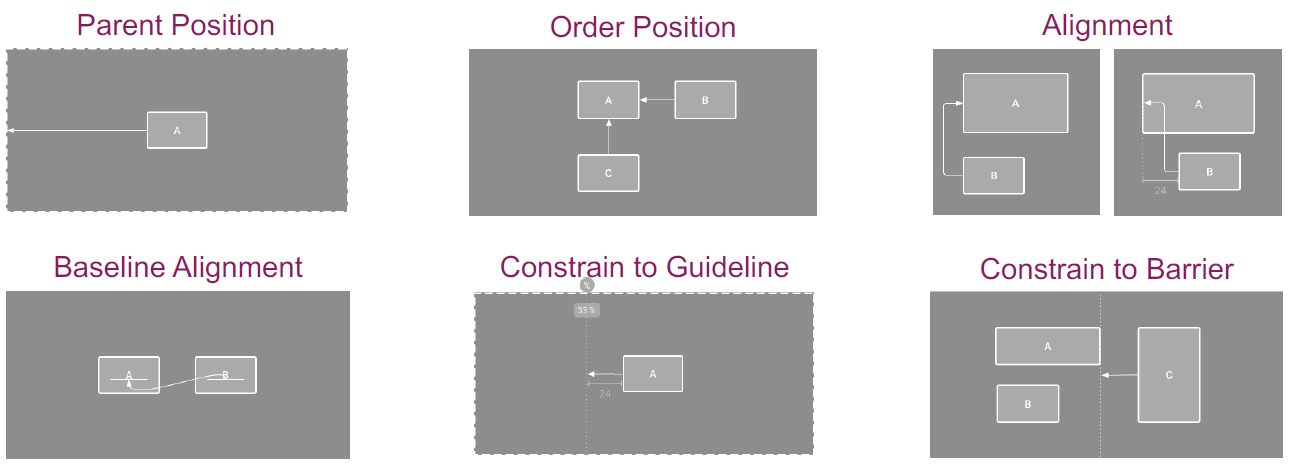
\includegraphics{layouts_constraint.png}
\subsection{Widgets}
\textbf{Namespace:} \textcolor{blue}{android.widget}\\
\textbf{Basisklasse:} \textcolor{blue}{View}
\subsubsection{TextView und ImageView}
\textbf{TextView zur Anzeige von Text:}
\begin{lstlisting}
<TextView
    ...
    android:text="TextView"
    android:textSize="20sp"
    android:textStyle="bold"
    android:typeface="monospace"
    android:textColor="@android:color/white"
    android:background="@color/colorPrimaryDark"
    android:drawableEnd="@drawable/ic_emoji"
    android:drawableTint="@android:color/white" />
\end{lstlisting}
\textbf{ImageView zur Anzeige von Bildern:}
\begin{lstlisting}
<ImageView
    ...
    android:layout_height="80dp"
    android:src="@drawable/ic_emoji"
    android:scaleType="fitCenter"
    android:tint="@color/colorPrimaryDark" />
\end{lstlisting}
\subsubsection{Button und ImageButton}
Buttons. Lösen via Listener Aktionen aus. Ableitung von TextView bzw. ImageView.
\begin{lstlisting}
<Button
    ...
    android:text="Button"
    android:drawableEnd="@drawable/ic_emoji"
    android:drawableTint="@color/colorPrimary"/>
\end{lstlisting}
\subsubsection{EditText}
EditText dient als Eingabefeld für Texte und Zahlen. \textcolor{blue}{android:inputType} beeinflusst Verhalten und aussehen (auch Keyboard).
\begin{lstlisting}
android:inputType="textPassword"
android:inputType="date"
android:inputType="textMultiLine"
// Auch kombinierbar
android:inputType="textCapCharacters|textAutoCorrect"
\end{lstlisting}
Bei der Texteingabe kann auf Ereignisse reagiert werden. Dazu muss ein TextWatcher als Listener registriert werden. Folgende 3 Methoden können überschrieben werden:
\begin{itemize}[topsep=0pt, leftmargin=4mm]
    \setlength\itemsep{-0.3em}
    \item beforeTextChanged
    \item onTextChanged
    \item afterTextChanged
\end{itemize}
\begin{lstlisting}
myEditText.addTextChangedListener(new TextWatcher() {
    public void afterTextChanged(Editable editable) {
        if (editable.length() < 8) {
            passwordInput.setError("Passwort zu kurz.");
        }
    }
})
\end{lstlisting}
\textbf{Weitere, häufig verwendete Widgets:}\\
Checkbox, Picker, Floating Action Button, Radio Buttons, Seek Bar, Spinner
\subsubsection{UI-Elemente ohne XML}
Werden direkt aus dem Code heraus erzeugt. Anpassbarkeit ist oft eingeschränkt (Farben, Texte, etc.)\\
\textbf{Toasts:} Einfache Rückmeldung zu Vorgang (Pop Up)\\
\textbf{Snackbars:} Wie Toast, aber mit Interaktion.\\
\textbf{Dialoge:} Erzwingen Aktion von Benutzer\\
\textbf{Notification:} Mitteilung ausserhalb aktiver Nutzung. NotificationCompat in AndroidX verwenden.\\
\textbf{Manus:} Existieren in verschiedenen Varianten. Options Menu, Contextual Menu, Popup Menu. $\rightarrow$ Wird generell als Resource in res/menu definiert.
\subsection{ScrollView}
\begin{itemize}[topsep=0pt, leftmargin=4mm]
    \setlength\itemsep{-0.3em}
    \item Ist ein spezielles Layout mit nur einem Kind-Element
    \item Erlaubt das vertikale Scrolling des Inhalts
    \item Horizontal nur mit \textcolor{blue}{HorizontalScrollView}
    \item Alternative in AndroidX: NestedScrollView (erlaubt beide Richtungen)
\end{itemize}
\begin{lstlisting}
<ScrollView
    android:layout_width="match_parent"
    android:layout_height="match_parent">
    <!-- Genau ein Kind hier -->
</ScrollView>
\end{lstlisting}
\subsection{ListView und ArrayAdapter}
Gut für Darstellung von Collections. Ein Adapter vermittelt zwischen der Darstellung und der Datenquelle.
\begin{lstlisting}
// main_activity.xml
<?xml version="1.0" encoding="utf-8"?>
<ListView xmlns:android="…"
    android:id="@+id/list_example"
    android:layout_width="match_parent"
    android:layout_height="match_parent">
</ListView>

// MainActivity.java
setContentView(R.layout.activity_main);
String[] data = new String[] { … };
ArrayAdapter<String> adapter = new ArrayAdapter<>(
    this,
    android.R.layout.simple_list_item_1,
    android.R.id.text1,
    data);
ListView listView = findViewById(R.id.list_example);
listView.setAdapter(adapter);
\end{lstlisting}
\subsection{RecyclerView}
Die RecyclerView ist eine moderne Alternative zu ListView und GridView. Ist Teil von AndroidX und erzwingt die Verwendung von View Holdern.
\begin{lstlisting}
// main_activity.xml
<?xml version="1.0" encoding="utf-8"?>
<androidx.recyclerview.widget.RecyclerView
    android:id="@+id/recycler_view"
    android:layout_width="match_parent"
    android:layout_height="match_parent">
</androidx.recyclerview.widget.RecyclerView>

// MainActivity.java
setContentView(R.layout.activity_recyclerview);
RecyclerView recyclerView = findViewById(R.id.recycler_view);
RecyclerView.LayoutManager layoutManager;
layoutManager = new LinearLayoutManager(this);
recyclerView.setLayoutManager(layoutManager);
ArrayList<User> data = UserManager.getUsers();
UsersAdapter adapter = new UsersAdapter(data);
recyclerView.setAdapter(adapter);

// UsersAdapter.java
public class UsersAdapter extends RecyclerView.Adapter<ViewHolder> {
    private ArrayList<User> users;

    @Override
    public ViewHolder onCreateViewHolder(ViewGroup parent, int vt) {
        Context context = parent.getContext();
        LayoutInflater inflater = LayoutInflater.from(context);

        View view = inflater.inflate(
            android.R.layout.simple_list_item_2,
            parent,
            false);

        return new ViewHolder(
            view,
            view.findViewById(android.R.id.text1),
            view.findViewById(android.R.id.text2));
    }

    @Override
    public void onBindViewHolder(ViewHolder holder, int position) {
        User user = this.users.get(position);
        holder.text1.setText(user.name);
        holder.text2.setText(user.age + " Jahre");
    }

    @Override
    public int getItemCount() {
        return this.users.size();
    }
}
\end{lstlisting}